%-----------------------------------------------------------------------------%
\chapter{\babTiga}
\label{chap:babTiga}
%-----------------------------------------------------------------------------%

Pada bab ini dijelaskan mengenai tahapan penelitian, seperti yang ditunjukkan pada Tabel \ref{tab:tahapan_penelitian}, yang meliputi studi literatur, perancangan dan implementasi sistem, serta evaluasi dan analisis.

\begin{table}
\centering
\caption{Tahapan penelitian}
\label{tab:tahapan_penelitian}
\begin{tabular}{p{3.5cm} p{4.5cm} p{4.5cm}}
\hline
\textbf{Tahapan} & \textbf{Alat} & \textbf{Hasil} \\
\hline
Studi literatur & Mesin pencari buku dan jurnal elektronik & Latar belakang masalah, rumusan masalah, rangkuman penelitian terkait dan ide rancangan sistem \\
\hline
Perancangan dan pengimplentasian sistem & Java, Python, Git, editor kode & Sistem Open IE \\
\hline
Evaluasi dan analisis & Python & Tabel hasil, diagram hasil, kesimpulan dan saran \\
\hline
\end{tabular}
\end{table}

%-----------------------------------------------------------------------------%
\section{Studi Literatur}
%-----------------------------------------------------------------------------%

Pada tahap ini \saya~mengumpulkan dan menelaah dokumen ilmiah seperti \textit{paper} dan artikel elektronik terkait \textit{open IE} untuk memahami topik ini secara lebih mendalam dan mengetahui pencapaian penelitian-penelitian terkait. Pencarian dilakukan digunakan menggunakan mesin pencari\footnote{Database Jurnal Universitas Indonesia \url{http://remote-lib.ui.ac.id}}\footnote{Google Scholar \url{https://scholar.google.co.id/}} jurnal dan artikel ilmiah elektronik nasional dan internasional. Hasil penelaahan ini berupa latar belakang dan rumusan masalah yang dituangkan pada bab \ref{chap:babSatu}, rangkuman dan perbandingan sistem \textit{open IE} pada bab \ref{chap:babDua}, serta ide rancangan sistem \textit{open IE} untuk bahasa Indonesia yang akan dijelaskan pada subbab berikutnya.

%-----------------------------------------------------------------------------%
\section{Rancangan dan Implementasi Sistem}
%-----------------------------------------------------------------------------%

Pada tahap ini \saya~merancang sistem \textit{open IE} untuk bahasa Indonesia yang mengadaptasi beberapa teknik pada sistem \textit{open IE} pada penelitian terkait. Rancangan sistem ini berisi empat modul utama, seperti yang ditunjukkan pada Gambar \ref{fig:program_flowchart}, yaitu \textbf{NLP pipeline}, \textbf{triple candidate generator}, \textbf{triple selector} dan \textbf{token expander}. Terdapat tiga fase atau langkah untuk melakukan ekstraksi \textit{triple} menggunakan sistem ini:

\begin{enumerate}
	\item Label (\textit{label}): membangun data latih untuk untuk \textit{triple selector} dengan menganotasi manual kandidat \textit{triple} yang dihasilkan oleh \textit{triple candidate generator} dan \textit{NLP pipeline}.  
	\item Belajar (\textit{learn}): melatih \textit{triple selector} untuk mengekstrak himpunan \textit{triple} dari kalimat menggunakan data dari fase Label. Hasil dari fase ini adalah model yang dipakai pada fase berikutnya.
	\item Ekstrak (\textit{extract}): mengekstrak himpunan \textit{triple} dari kalimat menggunakan \textit{NLP pipeline}, \textit{triple candidate generator}, \textit{token expander} dan \textit{triple selector} yang telah dilatih pada fase Belajar. Alur kerja pada fase ini ditunjukkan pada Gambar \ref{fig:program_flowchart}.
\end{enumerate}



\begin{figure}
\centering
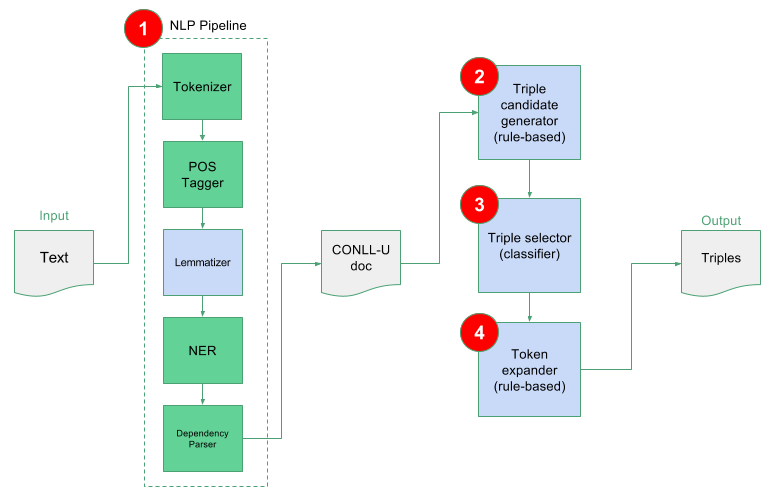
\includegraphics[width=\textwidth]{../images/program_flowchart.png}
\caption{Indonesian open domain information extraction flowchart}
\label{fig:program_flowchart}
\end{figure}

\subsection{NLP Pipeline}

\textit{NLP pipeline} adalah modul yang berisi serangkaian \textit{NLP task} yang menganotasi kalimat bahasa Indonesia dan menyimpannya sebagai dokumen dengan format CoNLL-U. Modul ini menerima dokumen teks yang berisi satu atau lebih kalimat yang dipisahkan oleh karakter baris baru (\textit{newline}) dan menghasilkan dokumen teks berisi kalimat yang telah dipotong menjadi \textit{token} dan diberi anotasi dengan format CoNLL-U. Rangkaian ini diimplementasikan menggunakan pustaka \textit{Stanford Core NLP}, seperti yang ditunjukkan pada berkas \verb|DependencyParser.java| pada lampiran, dan didistribusikan dalam format \textit{Java Archieve} (JAR) sehingga mudah dintegrasikan dengan modul lain. \textit{NLP task} yang terdapat pada rangkaian ini adalah sebagai berikut:

\begin{enumerate}

\item \textit{Tokenizer} \\
\textit{Tokenizer} yang digunakan pada rangkaian ini adalah yang disediakan pustaka \textit{Stanford Core NLP}, \verb|PTBTokenizer| \citep{manningptbtokenizer}. \textit{Tokenizer} berbasis aturan (\textit{rule-based}) ini mengikuti \textit{tokenizer} yang digunakan untuk menghasilkan \textit{Penn Treebank 3}\footnote{\textit{Penn Treebank 3} \url{https://catalog.ldc.upenn.edu/LDC99T42}} (\textit{treebank} bahasa Inggris). Meskipun \textit{tokenizer} ini menyediakan opsi untuk menyesuaikan proses dengan bahasa lain, di penelitian ini kami hanya menggunakan opsi standar untuk memotong kalimat berdasarkan \textit{whiteline} untuk mendapatkan \textit{token}.

\textit{Part of Speech Tagger} (\textit{POS tagger}) yang digunakan pada rangkaian ini adalah, \verb|MaxentTagger| \citep{toutanova2003feature}, yang juga merupakan bagian dari pustaka \textit{Stanford Core NLP}. \textit{POS tagger} berbasis \textit{multi-class logistic regression} ini dilatih dengan data yang diperoleh dengan mengekstraksi \textit{POS tag} dari 5.036 kalimat \textit{treebank} \textit{universal dependency} (UD) bahasa Indonesia\footnote{UD \textit{treebank} Indonesia \url{https://github.com/UniversalDependencies/UD_Indonesian}}. Hasil pengujian model \textit{POS tagger} ini, menggunakan 559 kalimat lain dari sumber yang sama, mencapai akurasi per token \textbf{93.68\%} dan akurasi per kalimat \textbf{63.91\%} (seluruh token dalam kalimat dianotasi dengan \textit{POS tag} yang benar).

\item \textit{Lemmatizer} \\
\textit{Lemmatizer} yang digunakan pada rangkaian ini diadaptasi dari \textit{lemmatizer} bahasa Indonesia berbasis aturan \citep{suhartono2014lemmatization} dan diberi nama \verb|IndonesianLemmaAnnotator|. Adaptasi dilakukan dengan melakukan perubahan berikut:

\begin{itemize}
\item Kemampuan untuk memproses tidak hanya kata tapi juga kalimat
\item Peningkatan kecepatan dengan penggunaan \textit{in-memory database}
\item Meningkatan \textit{reusability} dengan implementasi ulang menggunakan Java serta integrasi dengan pustaka \textit{Stanford Core NLP}
\end{itemize}

\textit{Lemmatizer} ini mencapai akurasi \textbf{99\%} saat diuji dengan 5.638 pasangan kata dan \textit{lemma} bahasa Indonesia dari \cite{suhartono2014lemmatization}.

\item \textit{Named-Entity Recognizer} (NER) \\
\textit{Named-entity recognizer} (NER) yang digunakan dalam rangkaian ini adalah \verb|CRFClassifier| \citep{finkel2005incorporating} dari pustaka \textit{Stanford Core NLP}. NER berbasis \textit{Conditional Random Field (CRF) sequence models} ini dilatih dan diuji menggunakan data yang didapatkan dari dua sumber, yaitu dari Fakultas Ilmu Komputer, Universitas Indonesia dan dari repositori kode publik\footnote{NER Indonesia \url{https://github.com/yusufsyaifudin/indonesia-ner}}. Data ini berisi kalimat-kalimat yang setiap \textit{token}-nya yang relevan sudah diberi anotasi dari lima kelas: \textit{Person}, \textit{Organization}, \textit{Quantity} dan \textit{Time}. Hasil pelatihan dengan 3.535 kalimat dan pengujian dengan 426 kalimat adalah model yang mencapai rata-rata presisi 0.86, \textit{recall} 0.85 dan \textit{F1-score} \textbf{0.86}.

\item \textit{Dependency Parser} \\
\textit{Dependency parser} yang digunakan dalam rangkaian ini adalah salah satu modul dalam pustaka \textit{Standford Core NLP}, yaitu \verb|nndep.DependencyParser| \citep{chen2014fast}. \textit{Dependency parser} ini berbasiskan jaringan syaraf tiruan (\textit{artificial neural network}) yang mempelajari pola transisi antar \textit{token} dalam kalimat dalam membentuk \textit{dependency tree}. Data yang digunakan untuk melatih dan menguji \textit{dependency parser} ini diperoleh dari \textit{treebank} \textit{universal dependency} (UD) bahasa Indonesia (sama dengan yang digunakan untuk \textit{POS tagger}). Model yang dihasilkan dengan melatih \textit{dependency parser} menggunakan 5.036 kalimat bahasa Indonesia ini mencapai nilai \textbf{70\%} UAS (\textit{Unlabeled Attachment Score}) dan \textbf{46\%} LAS (\textit{Labeled Attachment Score}) ketika diuji dengan 559 kalimat.

\end{enumerate}

Estimasi kinerja dari modul \textit{NLP pipeline} ini dihitung dari rata-rata kinerja \textit{POS tagger} (\textit{sentence accuracy}), \textit{NER} (\textit{F1-score}) dan \textit{dependency parser} (LAS), yaitu \textbf{65.30\%}. Kinerja \textit{tokenizer} dan \textit{lemmatizer} tidak diperhitungkan karena dianggap sudah terwakili oleh \textit{NLP task} yang lain. Hasil dari \textit{NLP pipeline} ini adalah dokumen berisi anotasi setiap kalimat dengan format CoNLL-U seperti contoh pada Gambar \ref{fig:conllu_example}. Dokumen ini menjadi input bagi modul \textit{triple candidate generator} yang akan dijelaskan berikutnya. 

\begin{figure}
\centering
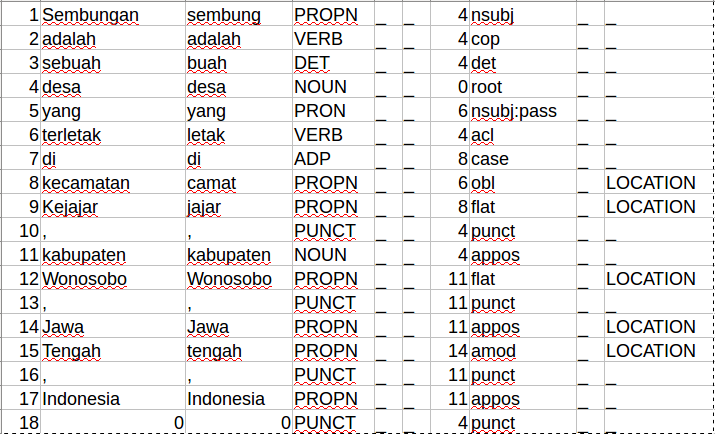
\includegraphics[width=\textwidth]{../images/conllu_example.png}
\caption{Contoh format CoNLL-U untuk sebuah kalimat}
\label{fig:conllu_example}
\end{figure}

\subsection{\textit{Triple Candidate Generator}} \label{Triple Candidate Generator}

Modul \textit{triple candidate generator} berfungsi untuk mengekstrak kandidat \textit{triple} dari dokumen CoNLL-U yang dihasilkan oleh \textit{NLP pipeline}. Modul ini menggunakan sejumlah aturan berbasis \textit{POS tag} dan \textit{dependency relation} yang ditampilkan pada Tabel \ref{tab:triple_candidate_generation_rules} untuk mengekstrak kandidat \textit{triple} dari tiap kalimat pada dokumen. Berbeda dengan \textsc{TextRunner} \citep{banko2007open} yang menghasilkan hanya menentukan kandidat yang valid secara otomatis, kandidat yang dihasilkan modul ini tidak semuanya valid sehingga diperlukan pelabelan oleh manusia (pada fase Label) atau pelabelan otomatis oleh \textit{classifier} (pada fase Extract) seperti pada \textsc{Stanford Open IE} \citep{angeli2015leveraging}. Modul ini diimplementasikan menggunakan bahasa pemrograman \textit{opensource} \textit{Python}\footnote{Python \url{https://www.python.org}} dengan fungsi utama \verb|extract_triples_by_combinations| pada berkas \verb|tripletools.py| yang disertakan pada lampiran.

% Triple candidate generation rules
\begin{table}
\renewcommand{\arraystretch}{1.5}
\caption{Aturan pembangkitan kandidat \textit{triple}}
\label{tab:triple_candidate_generation_rules}
\centering
\begin{tabular}{l p{12cm}}
\hline
\textbf{Jenis} & \textbf{Kondisi} \\
\hline
Subjek & \textit{POS tag} \textit{token} termasuk (PROPN, NOUN, PRON, VERB) \\
\space & \textit{Token} bukan termasuk ("yang", "adalah") \\
\space & \textit{Dependency} dari \textit{token} bukan termasuk ("compound", "name") \\
\space & \textit{Dependency} dari \textit{token} bukan termasuk ("compound", "name") tapi berjarak $>$ 2 dari \textit{head}-nya \\
\hline
Predikat & Posisi \textit{token} setelah Subjek \\
\space & \textit{POS tag} \textit{token} termasuk (VERB, AUX) \\
\hline
Objek & Posisi \textit{token} setelah Subjek dan Predikat \\
\space & \textit{POS tag} \textit{token} termasuk (PROPN, NOUN, PRON, VERB) \\
\space & \textit{Token} bukan termasuk ("yang", "adalah") \\
\space & \textit{Dependency} dari \textit{token} bukan termasuk ("compound", "name") \\
\space & \textit{Dependency} dari \textit{token} bukan termasuk ("compound", "name") tapi berjarak $>$ 2 dari \textit{head}-nya \\

\end{tabular}
\end{table}

Contoh aplikasi aturan \textit{triple candidate generator} pada contoh dokumen CoNLL-U pada Gambar \ref{fig:conllu_example} akan menghasilkan 17 kandidat \textit{triple} di mana hanya 5 di antaranya merupkan kandidat yang valid (ditandai dengan centang (\ding{51})):

\begin{itemize}
\item (Sembungan, adalah, desa) \ding{51}
\item (Sembungan, adalah, terletak)
\item (Sembungan, adalah, kecamatan)
\item (Sembungan, adalah, kabupaten)
\item (Sembungan, adalah, Jawa)
\item (Sembungan, adalah, Tengah)
\item (Sembungan, adalah, Indonesia)
\item (Sembungan, terletak, kecamatan) \ding{51}
\item (Sembungan, terletak, kabupaten) \ding{51}
\item (Sembungan, terletak, Jawa) \ding{51}
\item (Sembungan, terletak, Tengah)
\item (Sembungan, terletak, Indonesia) \ding{51}
\item (desa, terletak, kecamatan)
\item (desa, terletak, kabupaten)
\item (desa, terletak, Jawa)
\item (desa, terletak, Tengah)
\item (desa, terletak, Indonesia)
\end{itemize}

Untuk melatih modul \textit{triple selector} yang dapat memilih kandidat \textit{triple} yang valid, dibangun data pelatihan dengan melakukan pelabelan manual pada 1.611 kandidat \textit{triple} (132 positif dan 1479 negatif) yang dihasilkan \textit{triple candidate generator} dari 42 kalimat berformat CoNLL-U. Himpunan kalimat tersebut merupakan sebagian dari data \textit{universal dependency} Indonesia yang ditambahkan anotasi \textit{named-entity} secara manual.

Pada fase Ekstrak, \textit{triple candidate generator} juga digunakan untuk menghasilkan kandidat \textit{triple} dari dokumen CoNLL-U yang tidak berlabel seperti yang digambarkan pada Gambar \ref{fig:program_flowchart}. Hasil dari modul ini kemudian akan diseleksi oleh \textit{triple selector} yang telah dilatih pada fase Belajar. Lebih jauh mengenai \textit{triple} selector akan dijelaskan di subbab berikutnya.

\subsection{\textit{Triple Selector}}  \label{Triple Selector}

Modul \textit{triple selector} adalah sebuah \textit{supervised-learning classifier} yang dilatih untuk menyeleksi kandidat \textit{triple} yang dihasilkan oleh \textit{triple candidate generator}. Sebagai contoh, jika diberikan input 17 kandidat \textit{triple} yang disebutkan pada subbab \ref{Triple Candidate Generator}, modul ini akan mengambil lima kandidat \textit{triple} yang diberi tanda centang (\ding{51}) dan mengabaikan yang lainnya.

Metode yang digunakan untuk membangun \textit{classifier} pada modul ini adalah \textit{random forest} \citep{breiman2001random}, yang merupakan metode \textit{bagging} terhadap sejumlah \textit{decision tree}. Implementasi \textit{random forest} yang digunakan pada modul ini berasal dari pustaka \textit{scikit-learn}\footnote{scikit-learn \url{http://scikit-learn.org}} seperti yang ditunjukkan pada berkas \verb|classifier.py| (untuk fase Belajar) dan \verb|extract_triples.py| (untk fase Ekstrak) pada lampiran. Konfigurasi yang digunakan pada model \textit{random forest} pada modul ini adalah:

\begin{itemize}
\item Kriteria percabangan (\verb|criterion|): \textit{Gini Impurity}
\item Jumlah sampel minimal untuk membuat cabang  (\verb|min_samples_split|): 5
\item Jumlah fitur maksimum  (\verb|max_features|): 4 (akar dari jumlah total fitur)
\item Kedalaman maksimum  (\verb|max_depth|): 8
\item Jumlah pohon (\verb|n_estimators|): 20
\item Bobot kelas (\verb|class_weight|): \textit{balanced} (sesuai rasio kelas pada data)
\end{itemize}

Konfigurasi ini ditemukan dengan menggunakan algoritma \textit{grid search} \citep{wasserman2015grid}, algoritma pencarian menyeluruh (\textit{exhaustive}) terhadap sejumlah himpunan \textit{hyperparameter} untuk mengoptimalkan metrik evaluasi tertentu. Algoritma ini digunakan untuk mencari konfigurasi yang menghasilkan \textit{F1 score} terbaik untuk \textit{random forest} dengan data latih yang ada.

Untuk melakukan klasifikasi, 17 fitur berbasis \textit{POS tag}, \textit{named-entity} dan \textit{dependency relation} diekstrak dari masing-masing kandidat \textit{triple} dengan rincian pada Tabel \ref{tab:models_features}. Berbeda dengan \textsc{TextRunner} atau \textsc{ReVerb} \citep{banko2007open} \citep{etzioni2011open} yang lebih memilih menggunakan \textit{shallow syntactic features}, \textit{classifier} pada sistem ini menggunakan \textit{heavy linguistic features} seperti \textit{dependency relation} untuk mengoptimalkan \textit{precision} dan \textit{recall}.

\begin{table}
\caption{Fitur klasifikasi \textit{triple selector}}
\label{tab:models_features}
\centering
\begin{tabular}{r l}
\hline
\textbf{\#} & \textbf{Fitur Klasifikasi} \\
\hline
1 & \textit{POS tag} dari \textit{token} Subjek \\
2 & \textit{Dependency relation} dari \textit{token} Subjek \\
3 & \textit{POS tag} dari \textit{head} \textit{token} Subjek \\
4 & \textit{Named-entity} dari \textit{token} Subjek \\
5 & Jarak Subjek ke \textit{token} Predikat \\
6 & \textit{Dependency relation} dari \textit{token} Subjek ke Predikat \\
7 & \textit{POS tag} dari \textit{token} Predikat \\
8 & \textit{Dependency relation} dari \textit{token} Predikat \\
9 & \textit{POS tag} dari \textit{head} \textit{token} Predikat \\
10 & Jumlah \textit{dependents} \textit{token} Predikat \\
11 & \textit{POS tag} dari \textit{token} Objek \\
12 & \textit{Dependency relation} dari \textit{token} Objek \\
13 & \textit{POS tag} dari \textit{head} \textit{token} Objek \\
14 & \textit{Named-entity} dari \textit{token} Objek \\
15 & Jumlah \textit{dependents} dari \textit{token} Objek \\
16 & Jarak dari \textit{token} Objek ke predikat \\
17 & \textit{Dependency relation} \textit{token} Objek ke Predikat  \\
\end{tabular}
\end{table}

Pada fase Belajar, data kandidat \textit{triple} yang telah diberi label di fase Label diekstrak menjadi 17 fitur yang dijelaskan di Tabel \ref{tab:models_features} dan dinormalisasi menggunakan pustaka \verb|StandardScaler| dari \textit{sckit-learn}. Data fitur yang telah dinormalisasi tersebut dipakai untuk melatih \textit{classifier} dan hasilnya juga disimpan dalam berkas biner (\textit{binary file}) untuk digunakan pada fase Ekstrak.

\subsection{Token Expander}

Instead of using lightweight noun phrase chunker \citep{banko2007open}, our system uses rule-based token expander to extract relation or argument clauses. While having different objective and approach, this token expander works similarly to Clause Selector in Stanford Open IE \citep{angeli2015leveraging} where the algorithm starts from a token then decides whether to expand to its dependents. Instead of using machine learning model like Clause Selector, it uses simple heuristics based on syntactical features (POS tag, dependency relation and named-entity) described in Table \ref{tab:token_expansion_rules_s_o} and Table \ref{tab:token_expansion_rules_p} to determine whether to: (1) expand a token to its dependent, (2) ignore the dependent or (3) remove the token itself. For example, token expander will expand check-marked triples in Section \ref{Triple Candidate Generator} into:

\begin{itemize}
\item (Sembungan, adalah, desa)
\item (Sembungan, terletak di, kecamatan Kejajar)
\item (Sembungan, terletak di, kabupaten Wonosobo)
\item (Sembungan, terletak di, Jawa Tengah)
\item (Sembungan, terletak di, Indonesia)
\end{itemize}

% Token expansion rules for Subject or Object token
\begin{table}[!t]
\renewcommand{\arraystretch}{1.5}
\caption{Token expansion rules for Subject or Object token}
\label{tab:token_expansion_rules_s_o}
\centering
\begin{tabular}{r p{6cm} l}
\hline
\textbf{\#} & \textbf{Condition for Subject or Object Token} & \textbf{Action} \\
\hline
1 & If dependent's relation to the token  is either “compound”, “name”  or “amod” & Expand \\
2 & If dependent has same named entity as the token & Expand \\
3 & If dependent and the token are wrapped by quotes or double quotes  & Expand \\
4 & If the head is a sentence root & Ignore \\
5 & If dependent's POS tag is CONJ or its form is either “,” (comma) or “/” (slash) & Ignore \\
6 & If dependent's POS tag is either “VERB” or “ADP” & Ignore \\
7 & If dependent has at least one dependent with “ADP” POS tag & Ignore \\
8 & If the first or last token in expansion result has “CONJ” or “ADP” POS tag & Remove \\
9 & If the first or last index of expansion result is an incomplete parentheses symbol & Remove \\
10 & If the last index of expansion result is “yang” & Remove \\
11 & Else & Ignore \\
\hline
\end{tabular}
\end{table}

\begin{table}[!t]
\renewcommand{\arraystretch}{1.5}
\caption{Token expansion rules for Predicate token}
\label{tab:token_expansion_rules_p}
\centering
\begin{tabular}{r p{6cm} l}
\hline
\textbf{\#} & \textbf{Condition for Predicate Token} & \textbf{Action} \\
\hline
1 & If dependent is “tidak” & Expand \\
2 & Else & Ignore \\
\hline
\end{tabular}
\end{table}

During the label step, token expander is used to make manual annotation process easier. We label a triple candidate as valid only if it makes sense after being expanded to clause. For example, \textit{(Sembungan, terletak, kecamatan)} doesn't seem to make sense before expanded to \textit{(Sembungan, terletak di, kecamatan Kejajar)}.


%Kamus lemma \url{https://github.com/davidchristiandy/lemmatizer} (5,638 kata uji)
%
%Dataset POS tagging \url{https://github.com/UniversalDependencies/UD_Indonesian} (5,036 kalimat latih + 559 kalimat uji)
%
%Dataset NER Kelas NLP Fasilkom, UI, 2016 \url{https://github.com/yohanesgultom/knowledge-extractor-id} (1,700 kalimat latih  + 426 kalimat uji, 3 kelas entitas: Person, Organization, Location) \url{https://github.com/yusufsyaifudin/indonesia-ner} (1,835 kalimat latih, 5 kelas entitas: Person, Organization, Location, Quantity, Time)
%
%Dataset Dependency parsing \url{https://github.com/UniversalDependencies/UD_Indonesian} (5,036 kalimat latih + 559 kalimat uji)
%
%Dataset triple selector, anotasi manual dari sebagian dataset dependency parsing

%-----------------------------------------------------------------------------%
\section{Evaluasi dan Analisis}
%-----------------------------------------------------------------------------%

Untuk mengevaluasi kinerja dari algoritma \textit{supervised learning} dilakukan proses validasi silang (\textit{cross validation}) menggunakan data yang sudah diketahui kelasnya.